\clearpage
\pagestyle{fancy}
\part{Assi principali di inerzia}
\setcounter{section}{0}
\section{Formule di trasformazione}
%--------------------------------------------------------------------------------------------------------------------------------------------------------------
\renewcommand{\thefigure}{4~-~1}
\begin{figure}[ht]
\centering
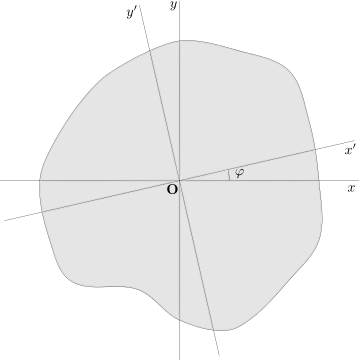
\includegraphics[width=0.65\textwidth]{Immagini/Parte_4/Figura4_1/Figura4_1.pdf}
\caption{}
\label{figura4-1}
\end{figure}
%--------------------------------------------------------------------------------------------------------------------------------------------------------------
\noindent Con riferimento alla figura~\ref{figura4-1}, ci poniamo il seguente quesito: 
%--------------------------------------------------------------------------------------------------------------------------------------------------------------
\begin{quoting}
Noti $I_x$, $I_y$ ed $I_{xy}$ è possibile ricavare $I_{x'}$, $I_{y'}$ ed $I_{x'y'}$?
\end{quoting}
%--------------------------------------------------------------------------------------------------------------------------------------------------------------
Ebbene, la risposta è affermativa, essendo valide le seguenti
%--------------------------------------------------------------------------------------------------------------------------------------------------------------
\begin{equation} \label{equazione4-1}
\boxed{\textup{\textsc{Formule di trasformazione}}} \longrightarrow
\begin{aligned}
I_{x'} &= I_{x}\cos^{2}\varphi+I_{y}\sin^{2}\varphi-I_{xy}\sin 2\varphi \\ 
I_{y'} &= I_{x}\sin^{2}\varphi+I_{y}\cos^{2}\varphi+I_{xy}\sin 2\varphi \\
I_{x'y'} &= \frac{I_{x}-I_{y}}{2}\sin 2\varphi+I_{xy}\cos 2\varphi
\end{aligned}
\tag{4.1}
\end{equation}
%--------------------------------------------------------------------------------------------------------------------------------------------------------------
Per una corretta utilizzazione delle~\eqref{equazione4-1} vale la pena sottolineare che
%--------------------------------------------------------------------------------------------------------------------------------------------------------------
\begin{enumerate}
\item i due riferimento $\mathbf{O}\,x\,y$ ed $\mathbf{O}\,x'\,y'$ devono avere in comune l'origine ed essere entrambi \textsc{ortogonali} e \textsc{levogiri};
\item $\varphi$ è l'angolo di cui $x'$ è ruotato rispetto ad $x$; esso deve essere misurato in senso antiorario, essendo ovviamente $0\le\varphi\le 2\pi$.
\end{enumerate}
%--------------------------------------------------------------------------------------------------------------------------------------------------------------
Le~\eqref{equazione4-1} si dimostrano agevolmente utilizzando le seguenti, ben note
%--------------------------------------------------------------------------------------------------------------------------------------------------------------
\begin{equation*}
\boxed{\textup{\textsc{Formule di trasformazione delle coordinate}}} \longrightarrow
\begin{aligned}
x' &= x\cos\varphi+y\sin\varphi \notag \\ 
y' &= -x\sin\varphi+y\cos\varphi \notag
\end{aligned}
\end{equation*}
%--------------------------------------------------------------------------------------------------------------------------------------------------------------
Dimostriamo, a titolo di esempio, solo la terza delle~\eqref{equazione4-1}:
%--------------------------------------------------------------------------------------------------------------------------------------------------------------
\begin{align*}
I_{x'y'} &= \int\int_A x'y'dA = \int\int_A (x\cos\varphi+y\sin\varphi)(-x\sin\varphi+y\cos\varphi)dA = \\
           &= \int\int_A (-x^{2}\sin\varphi\cos\varphi-xy\sin^{2}\varphi+xy\cos^{2}\varphi+y^{2}\sin\varphi\cos\varphi)dA
\end{align*}
%--------------------------------------------------------------------------------------------------------------------------------------------------------------
essendo $\varphi$ costante rispetto a $dA$ e tenendo presente che
%--------------------------------------------------------------------------------------------------------------------------------------------------------------
\begin{equation*}
\,\,\biggl\{\,\
\begin{aligned}
2\sin\varphi\cos\varphi &= \sin 2\varphi \\
\cos^{2}\varphi-\sin^{2}\varphi  &= \cos 2\varphi
\end{aligned}
\end{equation*}
%--------------------------------------------------------------------------------------------------------------------------------------------------------------
possiamo dunque scrivere
%--------------------------------------------------------------------------------------------------------------------------------------------------------------
\begin{align*}
I_{x'y'} &= \frac{1}{2}\sin 2\varphi\int\int_A y^{2}dA + \frac{1}{2}\sin 2\varphi\int\int_A x^{2}dA +\cos\varphi\int\int_{A}xydA= \\
           &=  I_{x}\frac{1}{2}\sin 2\varphi + I_{y}\frac{1}{2}\sin 2\varphi +I_{xy}\cos\varphi
\end{align*}
%--------------------------------------------------------------------------------------------------------------------------------------------------------------
che è quanto volevamo ottenere
%--------------------------------------------------------------------------------------------------------------------------------------------------------------
\section{Gli assi principali di inerzia}
%--------------------------------------------------------------------------------------------------------------------------------------------------------------
\renewcommand{\thefigure}{4~-~2}
\begin{figure}[ht]
\centering
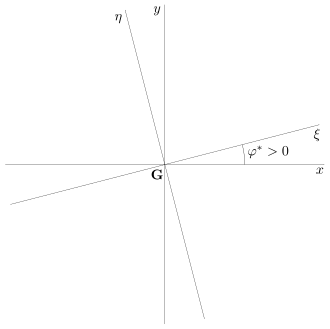
\includegraphics[width=0.65\textwidth]{Immagini/Parte_4/Figura4_2/Figura4_2.pdf}
\caption{}
\label{figura4-2}
\end{figure}
%--------------------------------------------------------------------------------------------------------------------------------------------------------------
\noindent Le equazioni~\eqref{equazione4-1} sono valide qualunque sia l'origine degli assi, ferme restando le precisazioni già fatte (si veda l'elenco della pagina precedente); naturalmente, esse acquistano la massima importanza allorché l'origine degli assi coincide con il baricentro. 

\noindent In ogni caso, dalle~\eqref{equazione4-1}, con semplici passaggi, si trae
%--------------------------------------------------------------------------------------------------------------------------------------------------------------
\begin{align*}
\frac{dI_{x'}}{d\varphi} &= -2I_{x'y'} \\
\frac{dI_{y'}}{d\varphi} &= +2I_{x'y'}
\end{align*}
%--------------------------------------------------------------------------------------------------------------------------------------------------------------
Da ciò scaturisce la seguente, notevole, proposizione
%--------------------------------------------------------------------------------------------------------------------------------------------------------------
\begin{quoting}
Tra gli infiniti riferimenti con origine in $\mathbf{G}$ ve ne è uno particolarmente importante, che indicheremo con $\mathbf{G}\xi\eta$. Si tratta di quel riferimento rispetto a cui è nullo il momento centrifugo e conseguentemente, i \textsc{momenti di inerzia} sono uno \textsc{minimo} e l'altro \textsc{massimo}.
\end{quoting}
%--------------------------------------------------------------------------------------------------------------------------------------------------------------
Le rette $\xi$ ed $\eta$ si dicono \textsc{assi principali di inerzia} della figura piana in esame. Esse sono baricentriche, ortogonali, e caratterizzate, come già detto, dalle condizioni seguenti
%--------------------------------------------------------------------------------------------------------------------------------------------------------------
\begin{align*}
I_{\xi} &= I_{\textup{max}}\,\textup{oppure}\,I_{\textup{min}} \\
I_{\eta} &= I_{\textup{max}}\,\textup{oppure}\,I_{\textup{min}} \\
I_{\xi\eta} &= 0
\end{align*}
%--------------------------------------------------------------------------------------------------------------------------------------------------------------
Dalla terza delle~\eqref{equazione4-1}, uguagliando a zero $I_{x'y'}$ si trova
%--------------------------------------------------------------------------------------------------------------------------------------------------------------
\begin{equation} \label{equazione4-2}
\boxed{\tan 2\varphi^* = \frac{2I_{xy}}{I_{y}-I_{x}}}
\tag{4.2}
\end{equation}
%--------------------------------------------------------------------------------------------------------------------------------------------------------------
Il valore di $\varphi^*$ che si ricava dalla~\eqref{equazione4-2} è l'angolo che $\xi$ forma con $x$; qualunque calcolatrice fornirà un valore di $2\varphi^*$ compreso fra $-90^{\circ}$ e $+90^{\circ}$; e quindi
%--------------------------------------------------------------------------------------------------------------------------------------------------------------
\begin{equation*}
\boxed{-45^{\circ}\le \varphi^{*} \le 45^{\circ}}
\end{equation*}
%--------------------------------------------------------------------------------------------------------------------------------------------------------------
La figura~\ref{figura4-2} mostra la corretta interpretazione grafica dell'asse $\xi$  e, conseguentemente, dell'asse $\eta$. Noto $\varphi^{*}$, è agevole calcolare $I_{\xi}$ ed $I_{\eta}$: basterà utilizzare le prime due delle~\eqref{equazione4-1} identificando $x'$ con $\xi$ ed $y'$ con $\eta$ e ponendo $\varphi^{*}$ al posto di $\varphi$. 

\noindent Noi sappiamo che
%--------------------------------------------------------------------------------------------------------------------------------------------------------------
\begin{equation*}
\boxed{r\textup{\textsc{ asse di simmetria (ortogonale o no) rispetto a }}\delta} \longrightarrow \boxed{I_{rs} = 0, \quad \forall\,s\parallelsum\,\delta}
\end{equation*}
%--------------------------------------------------------------------------------------------------------------------------------------------------------------
Ebbene, alla luce di quest'ultima proposizione, appaiono evidenti le seguenti:
%--------------------------------------------------------------------------------------------------------------------------------------------------------------
\begin{equation*}
\boxed{\textup{\scriptsize \textsc{Se una figura piana ha }}2\textup{\scriptsize \textsc{ assi di simmetria ortogonali, questi sono assi principali di inerzia}}}
\end{equation*}
%--------------------------------------------------------------------------------------------------------------------------------------------------------------
\begin{equation*}
\boxed{\textup{\scriptsize \textsc{Se una figura piana ha }}1\textup{\scriptsize \textsc{ asse di simmetria ortogonale, questo è asse principale di inerzia}}}
\end{equation*}
%--------------------------------------------------------------------------------------------------------------------------------------------------------------
Nel caso della seconda proposizione, l'altro asse è ovviamente ortogonale al primo e passante per $\mathbf{G}$.
%--------------------------------------------------------------------------------------------------------------------------------------------------------------
\clearpage
\section{Esercizi}
\paragraph{Esercizio 4.1}
Determinare gli assi principali di inerzia e calcolare i relativi momenti di inerzia per il profilato in figura.
%--------------------------------------------------------------------------------------------------------------------------------------------------------------
\renewcommand{\thefigure}{4.1~-~1}
\begin{figure}[ht]
\centering
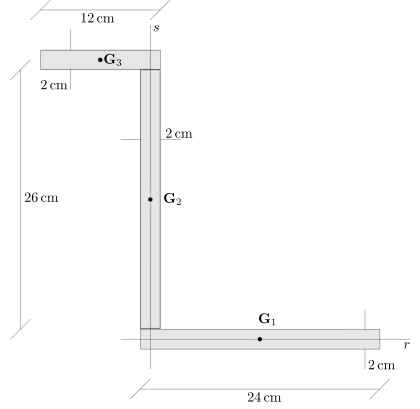
\includegraphics[width=0.8\textwidth]{Immagini/Parte_4/Esercizio4_1/Esercizio4_1_1.pdf}
\caption{}
\label{Esercizio4-1-1}
\end{figure}
%--------------------------------------------------------------------------------------------------------------------------------------------------------------

\noindent Cominciamo a determinare $\mathbf{G}$ 
%----------------------------------------------------------------------------------------
\begin{equation*}
\begin{aligned}
A_1 &= 48\,\textup{cm}^2 \\
A_2 &= 52\,\textup{cm}^2 \\
A_3 &= 24\,\textup{cm}^2
\end{aligned}
\,\,\Biggr\}\,\, A = 124\,\textup{cm}^2
\end{equation*}
%----------------------------------------------------------------------------------------
%----------------------------------------------------------------------------------------
\begin{equation*}
\begin{aligned}
S_{1r} &= 0\,\textup{cm}^3 \\
S_{2r} &= 54\times 14 = 728\,\textup{cm}^3 \\
S_{3r} &= 24\times 28  = 672\,\textup{cm}^3
\end{aligned}
\,\,\Biggr\}\,\, S_r = 1400\,\textup{cm}^3
\end{equation*}
%----------------------------------------------------------------------------------------
%----------------------------------------------------------------------------------------
\begin{equation*}
\begin{aligned}
S_{1s} &= 48\times 11 = 528\,\textup{cm}^3 \\
S_{2s} &= 0 \\
S_{3s} &= 24\times (-5)  = -120\,\textup{cm}^3
\end{aligned}
\,\,\Biggr\}\,\, S_r = 408\,\textup{cm}^3
\end{equation*}
%----------------------------------------------------------------------------------------
\begin{align*}
\lambda_{rG} &= \frac{S_r}{A} = \frac{1400}{124} = 11.29\,\textup{cm} \\
\lambda_{sG} &= \frac{S_s}{A} = \frac{408}{124} = 3.29\,\textup{cm}
\end{align*}
%----------------------------------------------------------------------------------------
%--------------------------------------------------------------------------------------------------------------------------------------------------------------
\renewcommand{\thefigure}{4.1~-~2}
\begin{figure}[ht]
\centering
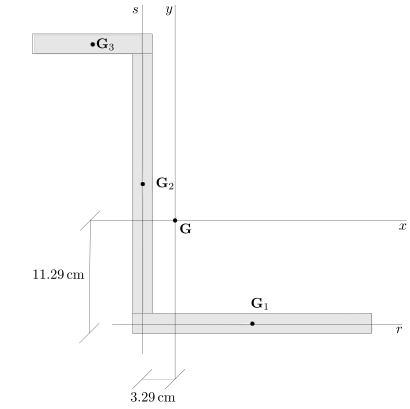
\includegraphics[width=0.8\textwidth]{Immagini/Parte_4/Esercizio4_1/Esercizio4_1_2.pdf}
\caption{}
\label{Esercizio4-1-2}
\end{figure}
%--------------------------------------------------------------------------------------------------------------------------------------------------------------

\noindent Abbiamo ridisegnato il profilato con gli assi $x$ ed $y$ paralleli ai lati dei rettangoli: questi sono, ovviamente, fra tutti gli assi baricentrici, quelli per cui è più agevole calcolare $I_x$, $I_y$ ed $I_{xy}$. Conviene comunque calcolare prima $I_r$, $I_s$ ed $I_{rs}$ per poi ricavare, applicando i teoremi del trasporto $I_x$, $I_y$ ed $I_{xy}$.
%----------------------------------------------------------------------------------------
\begin{equation*}
\begin{aligned}
I_{1r} &= \frac{24\times 2^3}{12} = 16\,\textup{cm}^4 \\
I_{2r} &= \frac{2\times 26^3}{12} + 52\times 14^2 = 13121\,\textup{cm}^4  \\
I_{3r} &= \frac{12\times 2^3}{12} + 24\times 28^2 = 18824\,\textup{cm}^4
\end{aligned}
\,\,\Biggr\}\,\, I_r = 31961\,\textup{cm}^4
\end{equation*}
%----------------------------------------------------------------------------------------
%----------------------------------------------------------------------------------------
\begin{equation*}
\begin{aligned}
I_{1s} &= \frac{2\times 26^3}{12} + 48\times 11^2 = 8112\,\textup{cm}^4 \\
I_{2s} &= \frac{26\times 2^3}{12} = 17\,\textup{cm}^4 \\
I_{3s} &= \frac{2\times 12^3}{12} + 24\times 5^2 = 888\,\textup{cm}^4
\end{aligned}
\,\,\Biggr\}\,\, I_s = 9017\,\textup{cm}^4
\end{equation*}
%----------------------------------------------------------------------------------------
%----------------------------------------------------------------------------------------
\begin{equation*}
\begin{aligned}
I_{1rs} &= 0 \\
I_{2rs} &= 0 \\
I_{3rs} &= 24\times(-5)\times 28 = -3360\,\textup{cm}^4
\end{aligned}
\,\,\Biggr\}\,\, I_{rs} = -3360\,\textup{cm}^4
\end{equation*}
%----------------------------------------------------------------------------------------
Ed ora possiamo calcolare $I_x$, $I_y$ ed $I_{xy}$
%----------------------------------------------------------------------------------------
\begin{align*}
I_{x} &= I_{r}-Ay_{G}^{2} = 31961-124\times 11.29^{2} = 16155\,\textup{cm}^4 \\
I_{y} &= I_{s}-Ax_{G}^{2} = 9017-124\times 3.29^{2} = 7675\,\textup{cm}^4  \\
I_{xy} &= I_{rs}-Ay_{G}x_{G} = -3360-124\times 11.29\times 3.29 = -7966\,\textup{cm}^4
\end{align*}
%----------------------------------------------------------------------------------------
A questo punto, applicando le~\eqref{equazione4-2}, possiamo calcolare l'angolo $\varphi^{*}$ che $\xi$ forma con $x$
%----------------------------------------------------------------------------------------
\begin{equation*}
\tan 2\varphi^{*} = \frac{2I_{xy}}{I_{y}-I_{x}} = -\frac{2\times 7966}{7675-16155} = 1.87877
\end{equation*}
%----------------------------------------------------------------------------------------
Quindi
%----------------------------------------------------------------------------------------
\begin{equation*}
2\varphi^{*} = 62^{\circ} \longrightarrow \varphi^{*} = 31^{\circ}
\end{equation*}
%--------------------------------------------------------------------------------------------------------------------------------------------------------------
\renewcommand{\thefigure}{4.1~-~3}
\begin{figure}[ht]
\centering
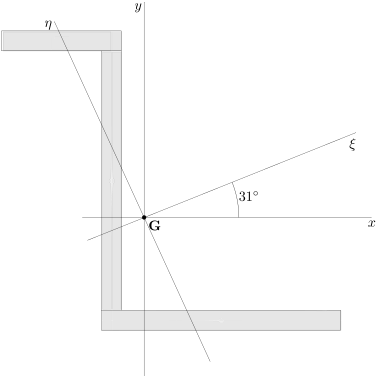
\includegraphics[width=\textwidth]{Immagini/Parte_4/Esercizio4_1/Esercizio4_1_3.pdf}
\caption{}
\label{Esercizio4-1-3}
\end{figure}
%--------------------------------------------------------------------------------------------------------------------------------------------------------------
Calcoleremo $I_{\xi}$ ed $I_{\eta}$ ponendo $\varphi=31^{\circ}$ rispettivamente nella prima e nella seconda delle~\eqref{equazione4-1}
%----------------------------------------------------------------------------------------
\begin{align*}
I_{\xi} &= 16155\times\cos^{2}31^{\circ}+7675\times\sin^{2}31^{\circ}+7966\times\sin^{2}62^{\circ} = 20939\,\textup{cm}^4 \\
I_{\eta} &= 16155\times\sin^{2}31^{\circ}+7675\times\cos^{2}31^{\circ}-7966\times\sin^{2}62^{\circ} = 2891\,\textup{cm}^4
\end{align*}
%----------------------------------------------------------------------------------------
La situazione finale ottenuta dal calcolo appena fatto è rappresentata in figura alla pagina seguente.
%----------------------------------------------------------------------------------------